\documentclass{article}
\usepackage[utf8]{inputenc}
\usepackage[spanish]{babel}
\usepackage{listings}
\usepackage{graphicx}
\graphicspath{ {images/} }
\usepackage{cite}

\begin{document}

\begin{titlepage}
    \begin{center}
        \vspace*{1cm}
            
        \Huge
        \textbf{Taller Calistenia}
            
        \vspace{0.5cm}
        \LARGE
        Informática II
            
        \vspace{1.5cm}
            
        \textbf{Reinaldo Marín Nieto}
            
        \vfill
            
        \vspace{0.8cm}
            
        \Large
        Despartamento de Ingeniería Electrónica y Telecomunicaciones\\
        Universidad de Antioquia\\
        Medellín\\
        Marzo de 2021
            
    \end{center}
\end{titlepage}

\tableofcontents
\newpage
\section{Descripción del ejercicio}\label{intro}
El ejercicio se basa en escribir una serie de instrucciones, para una tarea sencilla. La idea del mismo es que estas instrucciones sean muy específicas, pues servirán para que otras personas se guíen de éstos pasos para llevar una serie de objetos de un estado inicial a uno final.

\section{Ilustración del ejercicio} \label{contenido}
A continuación se presentan unas fotografías del estado inicial y final del sistema que se presenta en el ejercicio, de manera ilustrativa.
\subsection{Estado inicial}
\begin{figure}[h]
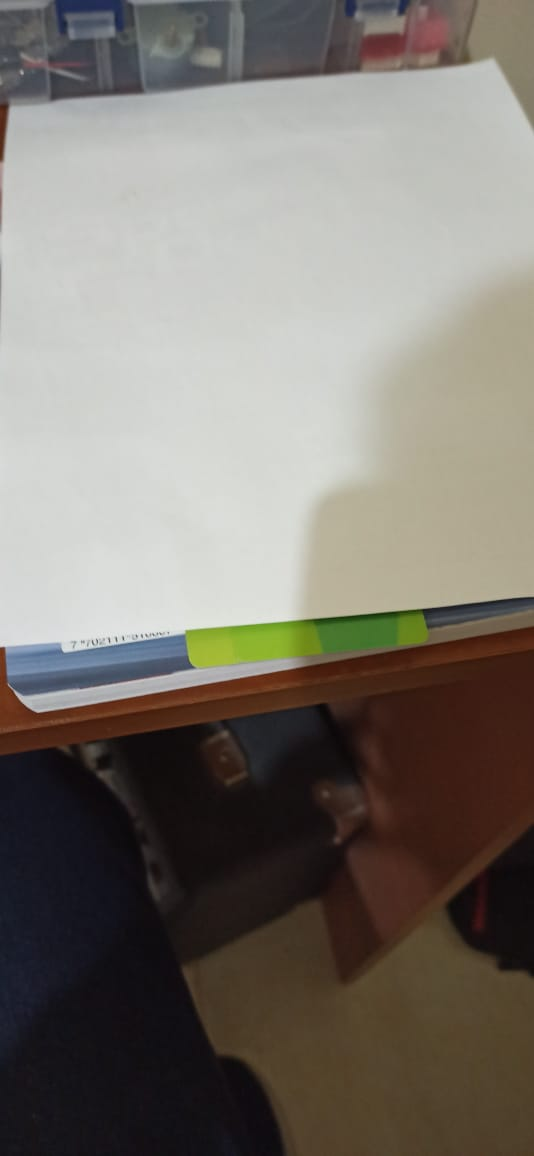
\includegraphics[width=4cm, height=4cm]{inicial.jpeg}
\centering
\caption{Estado inicial del sistema}
\label{fig:cpplogo}
\end{figure}
\subsection{Estado final}
\begin{figure}[h]
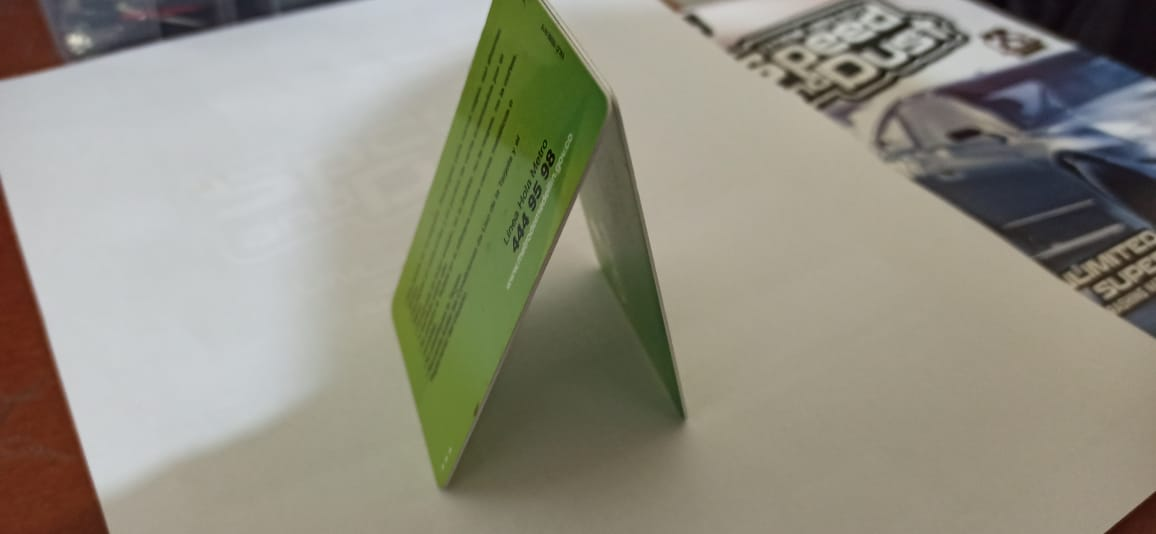
\includegraphics[width=4cm]{final.jpeg}
\centering
\caption{Estado final del sistema}
\label{fig:cpplogo}
\end{figure}
\newpage


\section{Método usado} \label{contenido}
Los pasos específicos para el desarrollo de la actividad se muestran a continuación:

Primero, levante la hoja de papel y hágala a un lado, luego tome las tarjetas. Toma las cartas entre el dedo índice y el dedo medio, de forma vertical, y pasa a introducir el dedo pulgar entre las dos tarjetas. Puede apoyar las tarjetas en la superficie de la hoja para evitar que caigan. Después de introducir el pulgar, súbalo un poco hasta que sólo las partes superiores de las tarjetas estén unidas, y las inferiores estén lo suficientemente separadas como para servir de base para la figura. Apoye esta figura triangular en la superficie de la mesa y súeltela cuando esté lo suficientemente equilibrada para mantenerse por si sola.

\section{Conclusión del ejercicio} 
Este ejercicio puede considerarse una demostración sobre lo tedioso que puede ser programar o dar órdenes sistemáticas específicas, sobretodo a los seres humanos, los cuales asumimos el paso siguiente, nos saltamos pasos o si nos guiamos de la ambigüedad, no llegamos a hacer ni la mitad de la acción. Nos muestra que para aprender a programar, primero necesitamos distribuir de manera estratégica y específica las acciones que queremos que realicen los programas.

Con nuestro primer sujeto, vimos que las tarjetas cayeron, pero en las instrucciones dadas nunca estuvo la condición de que se podían volver a levantar, por lo cuál el ejercicio terminó en ese instante. Ésto puede significar que muchas veces, debemos tener en cuenta todos los posibles caminos que puede tomar una ejecución, y planear una posible solución a todos los problemas que ésta pueda generar.



\end{document}
